\documentclass{BeamerTemplate}
\title{Module 4 - Quelques lois de probabilité continues et théorème central limite}
\subtitle{STT-1000 Probabilités et statistique}
\date{\today}

% Lien discret vers la page de réponses, ajouté au pied de page à côté du numéro
% (ne prend aucune place sur la diapo). Usage, n'importe où dans la diapo : \lienreponse{rep-ex}
\newcommand{\cibleReponse}{}
\newcommand{\lienreponse}[1]{\gdef\cibleReponse{#1}}
\addtobeamertemplate{footline}{}{%
  \ifx\cibleReponse\empty\else
    \begin{tikzpicture}[remember picture,overlay]
      \node[anchor=south east, inner sep=0pt] at ([xshift=-1.5cm,yshift=0.2cm]current page.south east)
        {\hyperlink{\cibleReponse}{\scriptsize\color{gray}Réponse~$\rightarrow$}};
    \end{tikzpicture}%
    \global\let\cibleReponse\empty
  \fi}
% Lien de retour vers l'exemple, dans les pages de réponses
\newcommand{\retour}[2]{\hyperlink{#1}{\textbf{#2}~{\color{gray}$\hookleftarrow$}}}

% Graphiques des densités et fonctions de répartition. Les styles sont définis
% ici, avant \begin{document} : babel-french rend « : » et « ; » actifs ensuite,
% ce qui briserait domain=0:5 dans les options d'un graphique.
\pgfplotsset{
  courbe/.style={
    width=6.6cm, height=5.4cm, axis lines=left, ymin=0,
    xlabel={$x$}, samples=121,
    tick label style={font=\tiny}, label style={font=\scriptsize},
    title style={font=\scriptsize\bfseries, yshift=-4pt},
    legend style={font=\tiny, draw=none, fill=none},
    legend cell align=left,
    scaled y ticks=false,
    yticklabel style={/pgf/number format/.cd, fixed, use comma},
    xticklabel style={/pgf/number format/.cd, use comma},
  },
  dom-exp/.style={domain=0:5},
  dom-gamma/.style={domain=0:5.2},
  dom-normale/.style={domain=-4:4},
  legende-haut/.style={legend pos=north east},
  legende-bas/.style={legend pos=south east},
  c1/.style={thick, color=blue!60!black, dashed},
  c2/.style={thick, color=teal!80!black},
  c3/.style={thick, color=red!65!black, dash dot},
  % fonctions de probabilité (quiz de l'urne)
  loi/.style={
    width=5.4cm, height=3.6cm, axis lines=left, ymin=0, ymax=0.5,
    tick label style={font=\tiny}, label style={font=\scriptsize},
    ylabel={Probabilité}, ylabel style={yshift=-2pt},
    ytick={0,0.1,0.2,0.3,0.4,0.5}, scaled y ticks=false,
    yticklabel style={/pgf/number format/.cd, fixed, fixed zerofill, precision=1, use comma},
  },
  urne1/.style={xmin=-0.2, xmax=3.3, xtick={0,1,2,3}},
  urne2/.style={xmin=-0.2, xmax=6.3, xtick={0,1,2,3,4,5,6}},
  baton/.style={ycomb, line width=2.2pt, color=red!75!black},
}

\begin{document}

\begin{frame}
\titlepage
\end{frame}

% ============================================================================
\section{Loi uniforme}

\begin{frame}[t]{Loi uniforme}

Il s'agit de la loi d'une variable aléatoire
\begin{itemize}
\item qui peut prendre toutes les valeurs d'un intervalle $[a,b]$;
\item dont tous les intervalles de même longueur sont \alerter{équiprobables}.
\end{itemize}
On note $X\sim\mathcal{U}(a,b)$.

\vspace{0.1in}
\textbf{Fonction de densité :}
$$f(x)=\left\{\begin{array}{ll}
\displaystyle \frac{1}{b-a}, & a\leq x\leq b\\
0, & \text{sinon.}
\end{array}\right.$$

{\small
\begin{align*}
E(X)=\frac{a+b}{2} & & V(X) = \frac{(b-a)^2}{12}
\end{align*}
}

\end{frame}


\begin{frame}[t]{Loi uniforme : espérance et variance}
Montrez les résultats pour $E(X)$ et $V(X)$.

\vspace{5cm}

\end{frame}


\begin{frame}[t]{Loi uniforme : fonction de répartition}

{\small
\begin{align*}
F(x)&=
\int_{-\infty}^xf(s)\;ds\\[10pt]
&= \left\{\begin{array}{ll}
\int_{-\infty}^x0\;ds, & x<a\\[6pt]
\int_{-\infty}^a 0\;ds+\int_a^x\frac{1}{b-a}\;ds, & a \le x<b\\[6pt]
\int_{-\infty}^a 0\;ds+\int_a^b\frac{1}{b-a}\;ds+\int_b^x0\;ds,
& x\ge b
\end{array}\right.\\[10pt]
&=\left\{\begin{array}{cl}
0, & x<a\\[6pt]
\frac{x-a}{b-a},  & a\le x<b\\[6pt]
1,& x\ge b.
\end{array}\right.
\end{align*}
}
\end{frame}


\begin{frame}[t,label=exfreq]{Fréquence d'un processeur}

{\small
Lors de l'exécution d'une tâche, la fréquence d'horloge demandée à un processeur
peut être n'importe quelle valeur entre 1,5 et 2 GHz, et toutes les valeurs de cet
intervalle sont équiprobables.

Quelle est la probabilité que la fréquence demandée dépasse 1,8 GHz?

\vspace{1in}
Quelle est l'espérance de la fréquence demandée?
}
\lienreponse{rep-ex1}
\end{frame}

% ============================================================================
\section{Loi exponentielle}

\begin{frame}[t]{Loi exponentielle}
Elle est liée à la loi de Poisson. Supposons que des événements surviennent selon un
\alerter{processus de Poisson de taux $\lambda$} (nombre moyen d'événements par unité de temps).
\begin{itemize}
\item Soit $Y$, le nombre d'événements dans un intervalle de temps de longueur $t$.
Alors $Y\sim\text{Poisson}(\lambda t)$.
\item Soit $X$, le \alerter{temps} qui s'écoule entre deux événements (ou avant le prochain événement).
\end{itemize}

\medskip
On peut montrer que $X$ suit une loi \alerter{exponentielle de taux $\lambda$}, notée $X\sim\text{Exp}(\lambda)$,
dont la densité est
$$f(x)=\left\{\begin{array}{ll}
\lambda e^{-\lambda x}, & x>0\\
0, & \text{sinon.}
\end{array}\right.$$
\end{frame}


\begin{frame}[t]{Loi exponentielle : espérance}

{\small
\begin{align*}
E(X)&=\int_{-\infty}^\infty x f(x)\;dx\\
&=\int_{-\infty}^0 x\cdot 0\;dx+\int_0^\infty x\lambda e^{-\lambda x}\;dx\\
(\text{posons\ }y=\lambda x)\ \ \ \ \
&=0+\frac{1}{\lambda}\int_{0}^{\infty}ye^{-y}\;dy\\
(\text{intégration par parties})\ \ \ \ \
&=\frac{1}{\lambda}\left\{\left[-ye^{-y}\right]_0^\infty+\int_0^\infty e^{-y}\;dy\right\}\\
&=\frac{1}{\lambda}
\end{align*}
}
\end{frame}


\begin{frame}[t]{Loi exponentielle : variance}

{\small
\begin{align*}
E(X^2)&=\int_{-\infty}^\infty x^2f(x)\;dx\\
&=\int_{-\infty}^0 x^2\cdot 0\;dx
+\int_0^\infty x^2\lambda e^{-\lambda x}\;dx\\
(\text{par parties, 2 fois})\ \ \ \ \ &=\frac{2}{\lambda^2}\\
&\ \ \\
\Rightarrow
V(X)&=E(X^2)-\{E(X)\}^2=\frac{2}{\lambda^2}-\left(\frac{1}{\lambda}\right)^2\\
&=\frac{1}{\lambda^2}
\end{align*}
}
\end{frame}


\begin{frame}[t]{Loi exponentielle : fonction de répartition}
\begin{align*}
F(x)&=\int_{-\infty}^xf(s)\;ds\\[10pt]
&=\left\{\begin{array}{ll}
\int_{-\infty}^x0\;ds, & x<0\\[6pt]
\int_{-\infty}^00\;ds+\int_0^x\lambda e^{-\lambda s}\;ds, & x\ge0
\end{array}\right.\\[10pt]
&=\left\{\begin{array}{ll}
0, & x<0\\[6pt]
1-e^{-\lambda x},  & x\ge0.
\end{array}\right.
\end{align*}
\end{frame}


\begin{frame}{Loi exponentielle : graphiques}

\begin{center}
\begin{tikzpicture}
\begin{axis}[courbe, dom-exp, legende-haut, name=g, ylabel={$f(x)$},
  title={Densité}, ymax=1.6]
  \addplot[c1] {0.5*exp(-0.5*x)}; \addlegendentry{$\lambda=0{,}5$}
  \addplot[c2] {exp(-x)};         \addlegendentry{$\lambda=1$}
  \addplot[c3] {1.5*exp(-1.5*x)}; \addlegendentry{$\lambda=1{,}5$}
\end{axis}
\begin{axis}[courbe, dom-exp, legende-bas, at={([xshift=0.9cm]g.outer east)}, anchor=outer west,
  ylabel={$F(x)$}, title={Fonction de répartition}, ymax=1.05]
  \addplot[c1] {1-exp(-0.5*x)}; \addlegendentry{$\lambda=0{,}5$}
  \addplot[c2] {1-exp(-x)};     \addlegendentry{$\lambda=1$}
  \addplot[c3] {1-exp(-1.5*x)}; \addlegendentry{$\lambda=1{,}5$}
\end{axis}
\end{tikzpicture}
\end{center}

\end{frame}


\begin{frame}[t,label=excommits]{Commits sur un dépôt}

{\small
Sur le dépôt Git d'un projet, le temps entre deux commits suit une loi exponentielle
de moyenne 3 heures. Quelle est la probabilité que plus de 6 heures s'écoulent entre
deux commits?

\vspace{1in} Quelle est la probabilité que 4 commits soient poussés en 15 heures?
}
\lienreponse{rep-ex1}
\end{frame}


\begin{frame}[t]{Loi exponentielle : absence de mémoire}
La loi exponentielle est \alerter{la seule loi continue sans mémoire} : pour tous $x,s>0$,
$$P(X>x+s\,|\,X>s)=P(X>x).$$
{\small Sachant qu'on a déjà attendu $s$, la probabilité d'attendre encore au moins $x$ ne
dépend pas de $s$. Par exemple, $P(X>10\,|\,X>6)=P(X>4)$.}

{\small
\begin{align*}
P(X>x+s\,|\,X>s)&=\frac{P(X>x+s\text{\ et\ }X>s)}{P(X>s)}
=\frac{P(X>x+s)}{P(X>s)}
=\frac{1-F_X(x+s)}{1-F_X(s)}\\[6pt]
&=\frac{1-\{1-\exp(-\lambda\{x+s\})\}}
{1-\{1-\exp(-\lambda s)\}}=\frac{\exp(-\lambda\{x+s\})}{\exp(-\lambda s)}\\[6pt]
&=e^{-\lambda x-\lambda s -(-\lambda s)} =e^{-\lambda x}
=1-(1-e^{-\lambda x})=P(X>x)
\end{align*}
}
\end{frame}


\begin{frame}[t,label=exserveur]{Serveur sans plantage}

{\small
La loi exponentielle est souvent utilisée pour modéliser le temps de fonctionnement
d'un système avant une panne. Le temps avant qu'un certain serveur plante suit une loi
exponentielle de moyenne 1000 heures. Ce serveur fonctionne déjà sans interruption depuis
500 heures. Quelle est la probabilité qu'il fonctionne encore au moins 1000 heures de plus?
}
\lienreponse{rep-ex1}
\end{frame}

% ============================================================================
\section{Loi Gamma}

\begin{frame}[t]{Loi Gamma}
Considérons $Y_1,\ldots,Y_n$ des variables aléatoires indépendantes et identiquement distribuées (i.i.d.),
telles que $Y_i\sim \text{Exp}(\lambda)$ pour $i =1,\ldots,n$. Alors
$$ X=\sum_{i=1}^nY_i  \sim \alerter{\text{Gamma}(n,\lambda)}.$$

\textbf{Fonction de densité :} si $X \sim \text{Gamma}(n,\lambda)$, où $n>0$ et $\lambda > 0$,
$$f(x)=\left\{\begin{array}{ll}
\dfrac{\lambda}{\Gamma(n)}(\lambda x)^{n-1}e^{-\lambda x}, & x > 0\\[6pt]
0, & \text{sinon.}
\end{array}\right.$$
{\small $\Gamma(\cdot)$ est la fonction Gamma, un peu complexe en général; pour un entier $n$, $\Gamma(n) = (n-1)!$}

\vspace{0.15in}
\textbf{Fonction de répartition :} pas de forme explicite.

\end{frame}


\begin{frame}{Loi Gamma : graphique}

\begin{center}
\begin{tikzpicture}
\begin{axis}[courbe, dom-gamma, legende-haut, width=8cm, height=5.4cm,
  ylabel={$f(x)$}, title={Densité de la loi Gamma$(n,\lambda)$}, ymax=1.05]
  \addplot[c1] {exp(-x)};           \addlegendentry{$n=1$, $\lambda=1$}
  \addplot[c2] {x*exp(-x)};         \addlegendentry{$n=2$, $\lambda=1$}
  \addplot[c3] {x*x*exp(-x)/2};     \addlegendentry{$n=3$, $\lambda=1$}
\end{axis}
\end{tikzpicture}
\end{center}

{\small Avec $n=1$, on retrouve la loi exponentielle.}
\end{frame}


\begin{frame}[t]{Loi Gamma : espérance et variance}

\textbf{Espérance :}
$$E(X)=E(Y_1+\cdots+Y_n)=\sum_{i=1}^nE(Y_i)=
 \sum_{i=1}^n\frac{1}{\lambda}=\frac{n}{\lambda}$$

\textbf{Variance :} les $Y_i$ sont indépendantes, donc $\text{Cov}(Y_i,Y_j)=0$ pour $i\neq j$ :
\begin{align*}
V(X)&=V(Y_1+\cdots+Y_n)\\
&=\sum_{i=1}^nV(Y_i)+2\sum\sum_{i<j}\text{Cov}(Y_i,Y_j)\\
&=\sum_{i=1}^n\frac{1}{\lambda^2}+2\sum\sum_{i<j}0= \frac{n}{\lambda^2}
\end{align*}

\end{frame}


\begin{frame}[t]{Lien avec les processus de Poisson}

Si des événements surviennent selon un processus de Poisson de taux $\lambda$, alors
\begin{itemize}\itemsep6pt
 \item le nombre d'événements dans un intervalle de longueur $t$
 suit une loi de Poisson de moyenne $\mu=\lambda t$;
 \item le temps avant le prochain événement (ou entre deux événements consécutifs)
 suit une loi exponentielle de taux $\lambda$, donc de moyenne $1/\lambda$;
 \item le temps avant le $n$-ième événement (ou entre un événement et le $n$-ième
 suivant) suit une loi Gamma$(n,\lambda)$.
\end{itemize}

\end{frame}


\begin{frame}[t]{En image}

{\small Des événements ($\times$) surviennent selon un processus de Poisson de taux $\lambda$ par unité de temps.}

\vspace{2.2cm}
\begin{center}
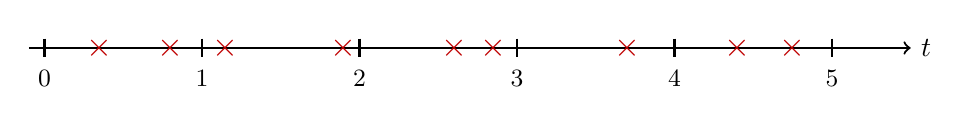
\begin{tikzpicture}[x=2cm]
  \draw[->, thick] (-0.1,0) -- (5.5,0) node[right] {$t$};
  \foreach \k in {0,...,5} {
    \draw[thick] (\k,0.12) -- (\k,-0.12) node[below=1pt] {\small $\k$};
  }
  \foreach \e in {0.35,0.8,1.15,1.9,2.6,2.85,3.7,4.4,4.75} {
    \node[red!75!black] at (\e,0) {\large$\times$};
  }
\end{tikzpicture}
\end{center}

\end{frame}


\begin{frame}[t,label=expirate]{Pirate informatique}

{\small
Les temps que prend un pirate informatique pour craquer des mots de passe peuvent
être vus comme des v.a. indépendantes de loi exponentielle de moyenne 15 minutes.
Quels sont la loi, la moyenne et la variance du temps qu'il lui faudra pour craquer
les trois mots de passe qui protègent un certain site?}
\lienreponse{rep-ex1}
\end{frame}


\begin{frame}[t]{Pirate informatique (suite)}

{\small
Si ce pirate dispose de 20 minutes, quelle est la probabilité qu'il craque exactement
2 mots de passe?
}
\lienreponse{rep-ex1}
\end{frame}

% ============================================================================
\section{Loi normale}

\begin{frame}[t]{Loi normale}

\vspace{0.1in}
La loi normale est probablement la loi de probabilité la plus utilisée dans les
applications de la statistique. Quelques raisons de sa popularité :
\vspace{0.1in}
\begin{itemize}
\item elle modélise bien la distribution de beaucoup de variables d'intérêt;
\item elle approxime la loi de plusieurs variables aléatoires de nature complexe (théorème central limite);
\item elle mène à des résultats analytiques dans plusieurs problèmes d'inférence statistique.
\end{itemize}
\end{frame}


\begin{frame}[t]{Loi normale}

La loi normale est définie par son espérance et sa variance.

\vspace{0.5in}
Si $X$ suit une loi normale d'espérance $\mu$ et de variance $\sigma^2$, notée
$X\sim \mathcal{N}(\mu,\sigma^2)$, alors
$$f(x)=\frac{1}{\sqrt{2\pi\sigma^2}}
e^{-\frac{1}{2}\left(\frac{x-\mu}{\sigma}\right)^2},\ \
-\infty<x<\infty.$$

\vspace{0.1in}
Comme le nom des paramètres l'indique, on a alors
$$E(X) = \mu \qquad \text{et} \qquad V(X) = \sigma^2.$$

\end{frame}


\begin{frame}{Loi normale : graphique}
\begin{center}
\begin{tikzpicture}
\begin{axis}[courbe, dom-normale, legende-haut, width=7.4cm, height=5.2cm,
  ylabel={$f(x)$}, title={Densité de la loi $\mathcal{N}(\mu,\sigma^2)$}, ymax=0.5,
  xtick={-4,-2,0,2,4}, legend style={at={(1.02,1)}, anchor=north west}]
  \addplot[c2] {exp(-x*x/2)/sqrt(2*pi)};         \addlegendentry{$\mathcal{N}(0,1)$}
  \addplot[c1] {exp(-x*x/4)/sqrt(4*pi)};         \addlegendentry{$\mathcal{N}(0,2)$}
  \addplot[c3] {exp(-(x-2)*(x-2)/4)/sqrt(4*pi)}; \addlegendentry{$\mathcal{N}(2,2)$}
\end{axis}
\end{tikzpicture}
\end{center}

\end{frame}


\begin{frame}[t]{Loi normale : propriétés de la densité}

\vspace{0.2in}
\begin{itemize}\itemsep10pt
\item $f(x)\ge0$ pour tout $x\in\mathbb{R}$
\item $\lim\limits_{x\to -\infty}f(x)=0$ et $\lim\limits_{x\to\infty}f(x)=0$
\item $f(\mu-x)=f(\mu+x)$ pour tout $x\in\mathbb{R}$, donc cette densité
est \alerter{symétrique autour de $\mu$}; en particulier, $P(X<\mu)=P(X>\mu)=1/2$ :
$\mu$ est aussi la médiane
\item $f(x)$ atteint son unique maximum en $x=\mu$
\item $f(x)$ a deux points d'inflexion, un en $\mu-\sigma$ et un en $\mu+\sigma$ (la deuxième dérivée y est nulle)
\end{itemize}
\end{frame}


\begin{frame}[t]{Loi normale : fonction de répartition}

\vspace{0.2in}
Rappel : si $X\sim \mathcal{N}(\mu,\sigma^2)$, alors
$$f(x)=\frac{1}{\sqrt{2\pi\sigma^2}}
e^{-\frac{1}{2}\left(\frac{x-\mu}{\sigma}\right)^2},\ \
-\infty<x<\infty.$$

Donc
$$ F(x) = \int_{-\infty}^x \frac{1}{\sqrt{2\pi\sigma^2}}
e^{-\frac{1}{2}\left(\frac{t-\mu}{\sigma}\right)^2} dt.$$

\vspace{0.2in}
Cette intégrale n'a pas de solution analytique. On obtient ses valeurs à l'aide d'un logiciel
(par exemple \texttt{R}, avec \texttt{pnorm}) ou d'une table.

\end{frame}


\begin{frame}[t]{Loi normale standard}

La loi $\mathcal{N}(0,1)$ est appelée \alerter{loi normale standard} ou encore \alerter{loi normale centrée réduite}.
Cette loi est très importante et mérite donc une notation spéciale.

\vspace{0.1in}
Si $Z \sim \mathcal{N}(0,1)$, on note
\begin{itemize}\itemsep8pt
\item  $\phi(z)$ la densité de $Z$ :
$\phi(z)=(2\pi)^{-1/2}e^{-z^2/2}$;
\item $\Phi(z)=P(Z\le z)$ la fonction de répartition de $Z$. \\[4pt]
$\Phi(z)$ n'a toujours pas de forme analytique, mais les livres de statistique contiennent une table des valeurs de $\Phi(z)$.
\end{itemize}

\end{frame}


% Table découpée en deux diapos (z de 0 à 1,99 puis de 2 à 3,99) pour rester lisible ;
% l'en-tête de la table est repris sur la deuxième.
\begin{frame}[t]{Table de la loi normale standard (1/2)}

\vspace{-0.3cm}
\begin{center}
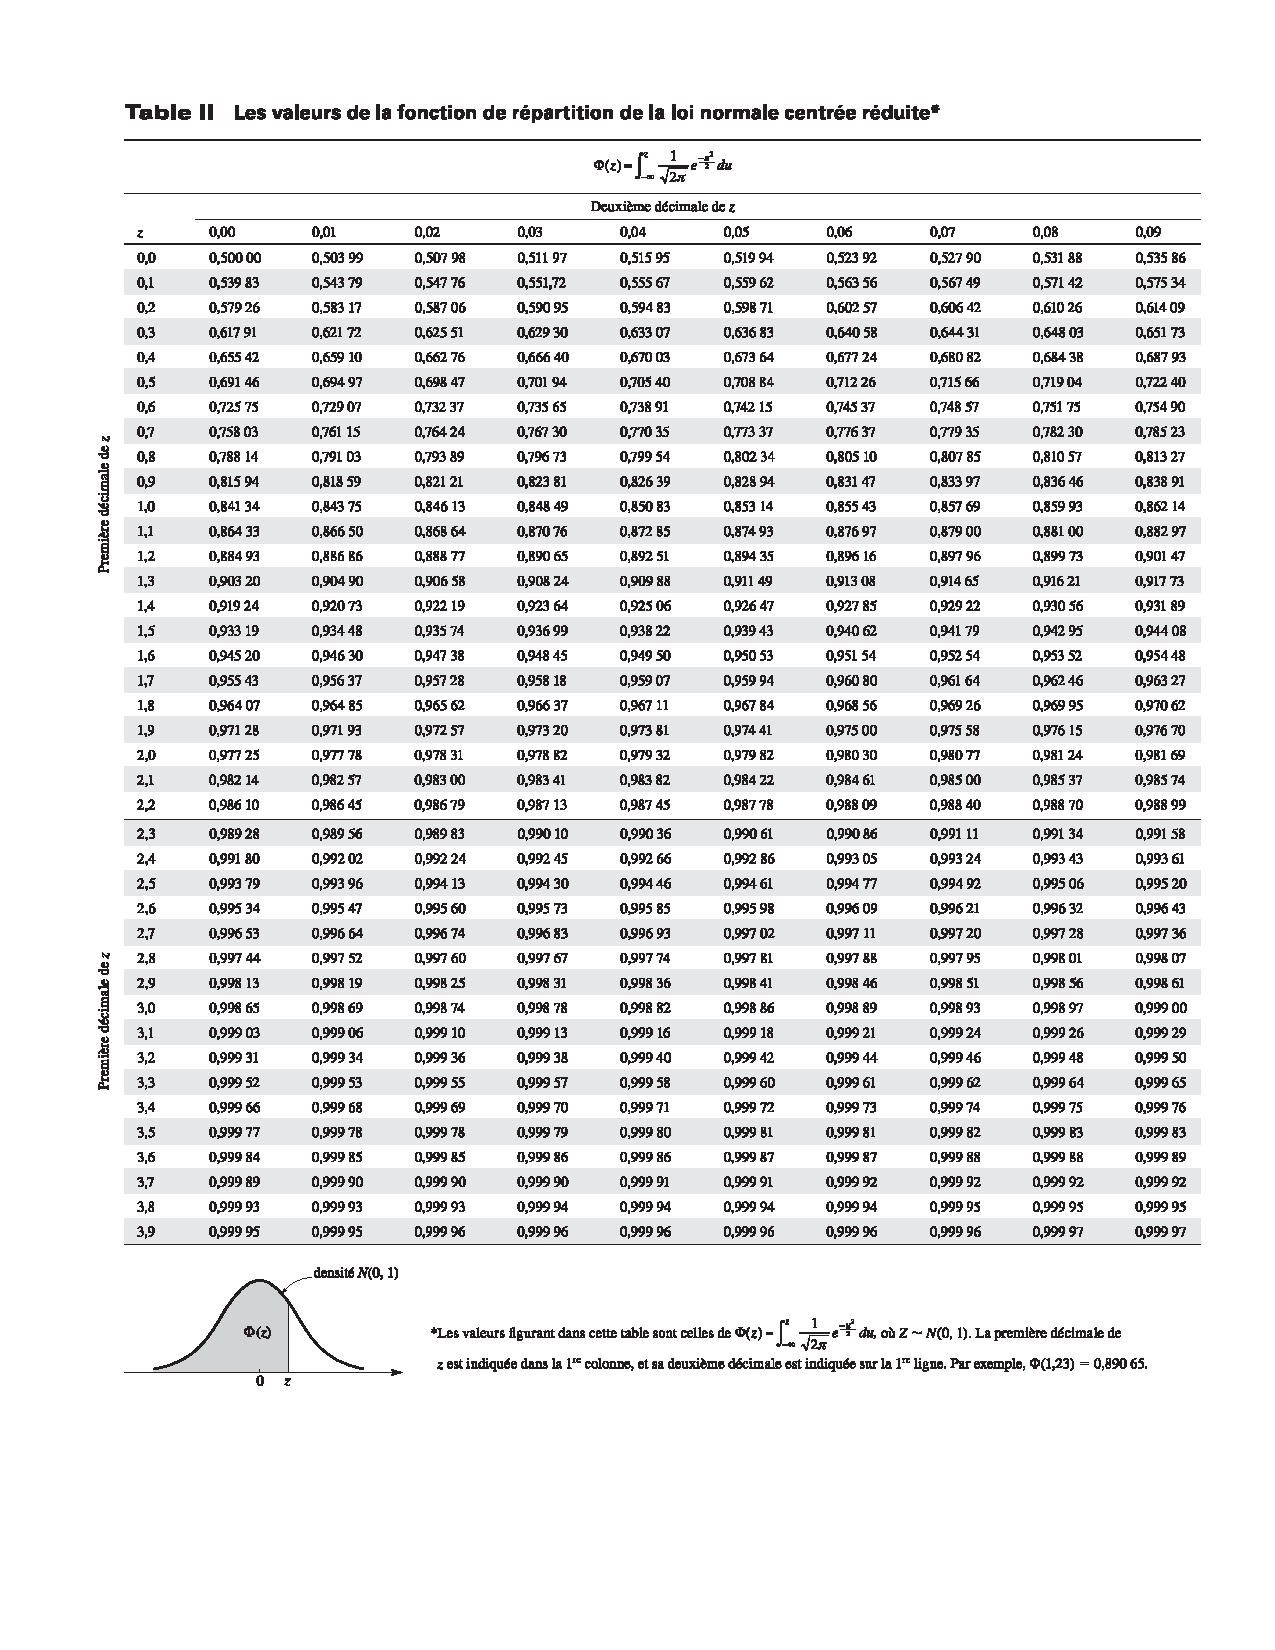
\includegraphics[trim=58 434 34 64, clip, scale=0.68]{TableNormale.pdf}
\end{center}

\end{frame}


\begin{frame}[t]{Table de la loi normale standard (2/2)}

\vspace{-0.3cm}
\begin{center}
\offinterlineskip
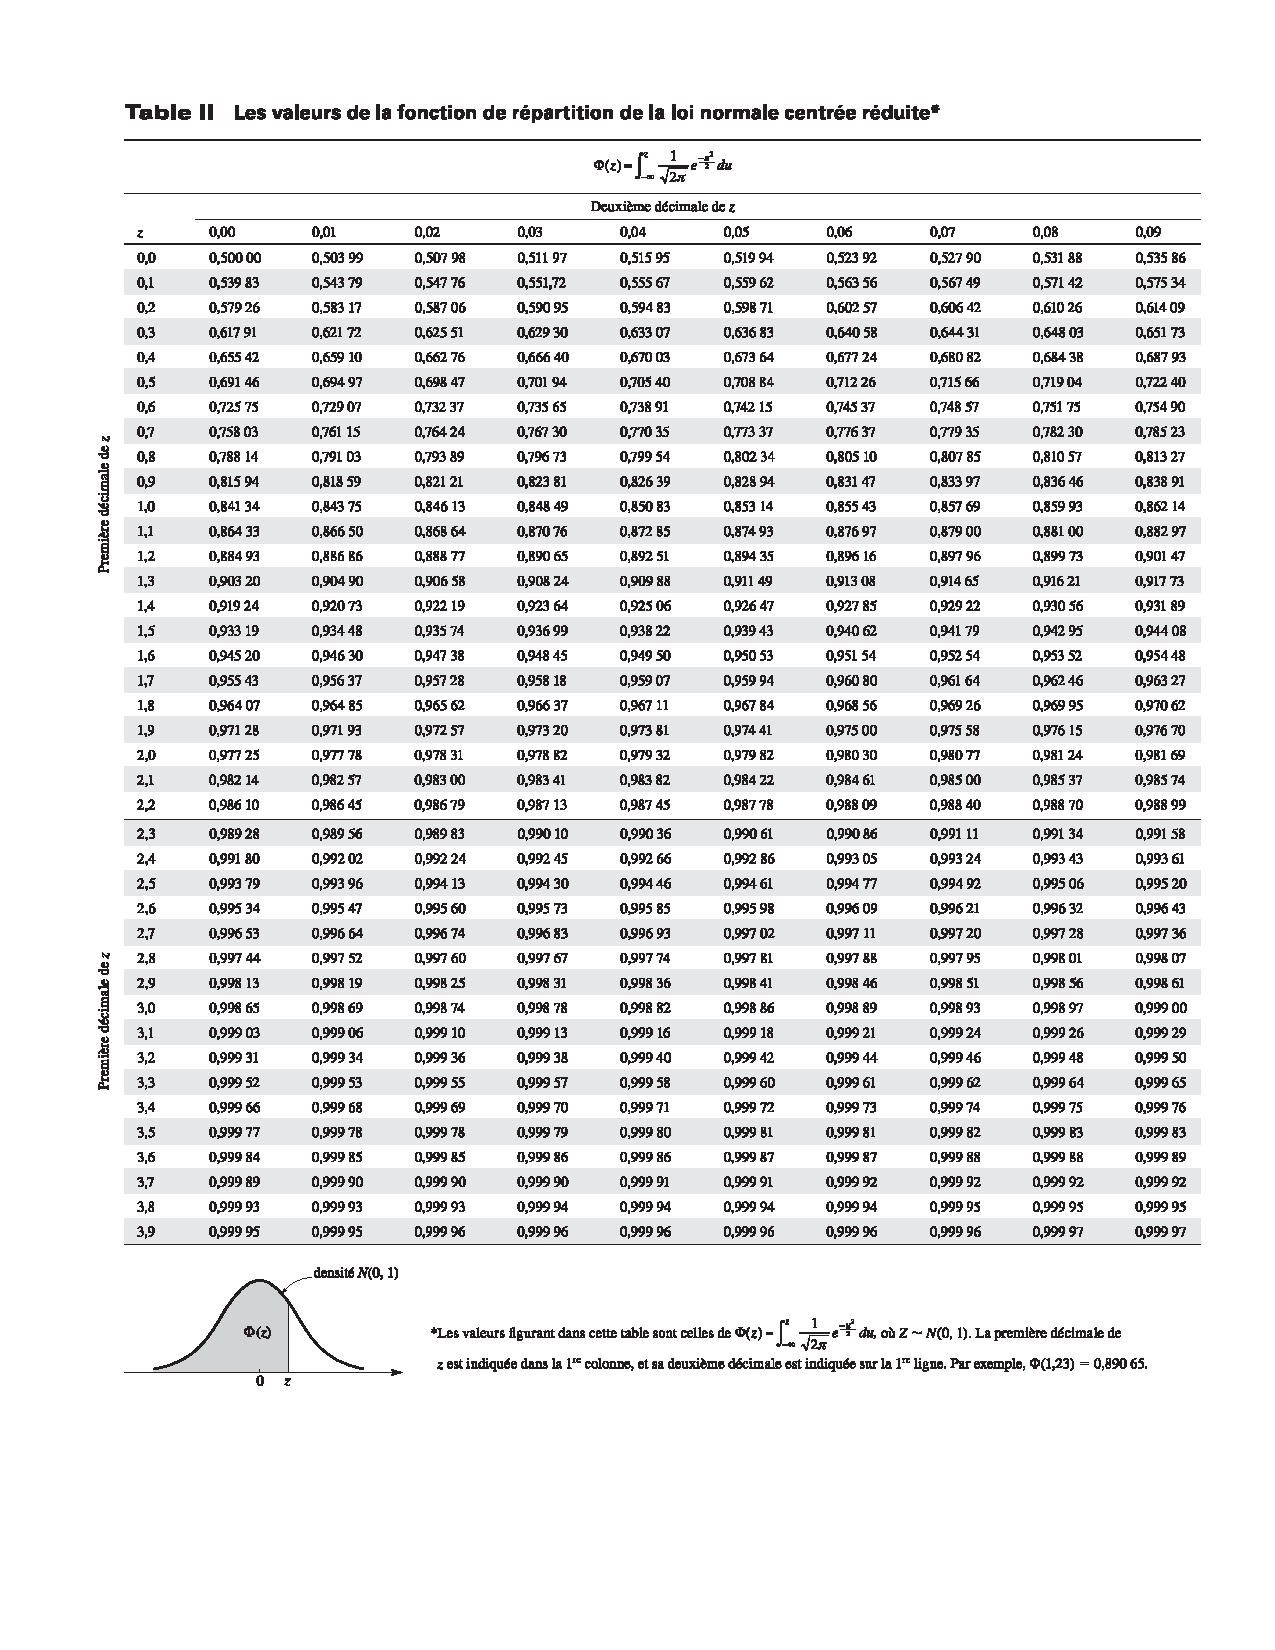
\includegraphics[trim=58 673 34 64, clip, scale=0.68]{TableNormale.pdf}\par
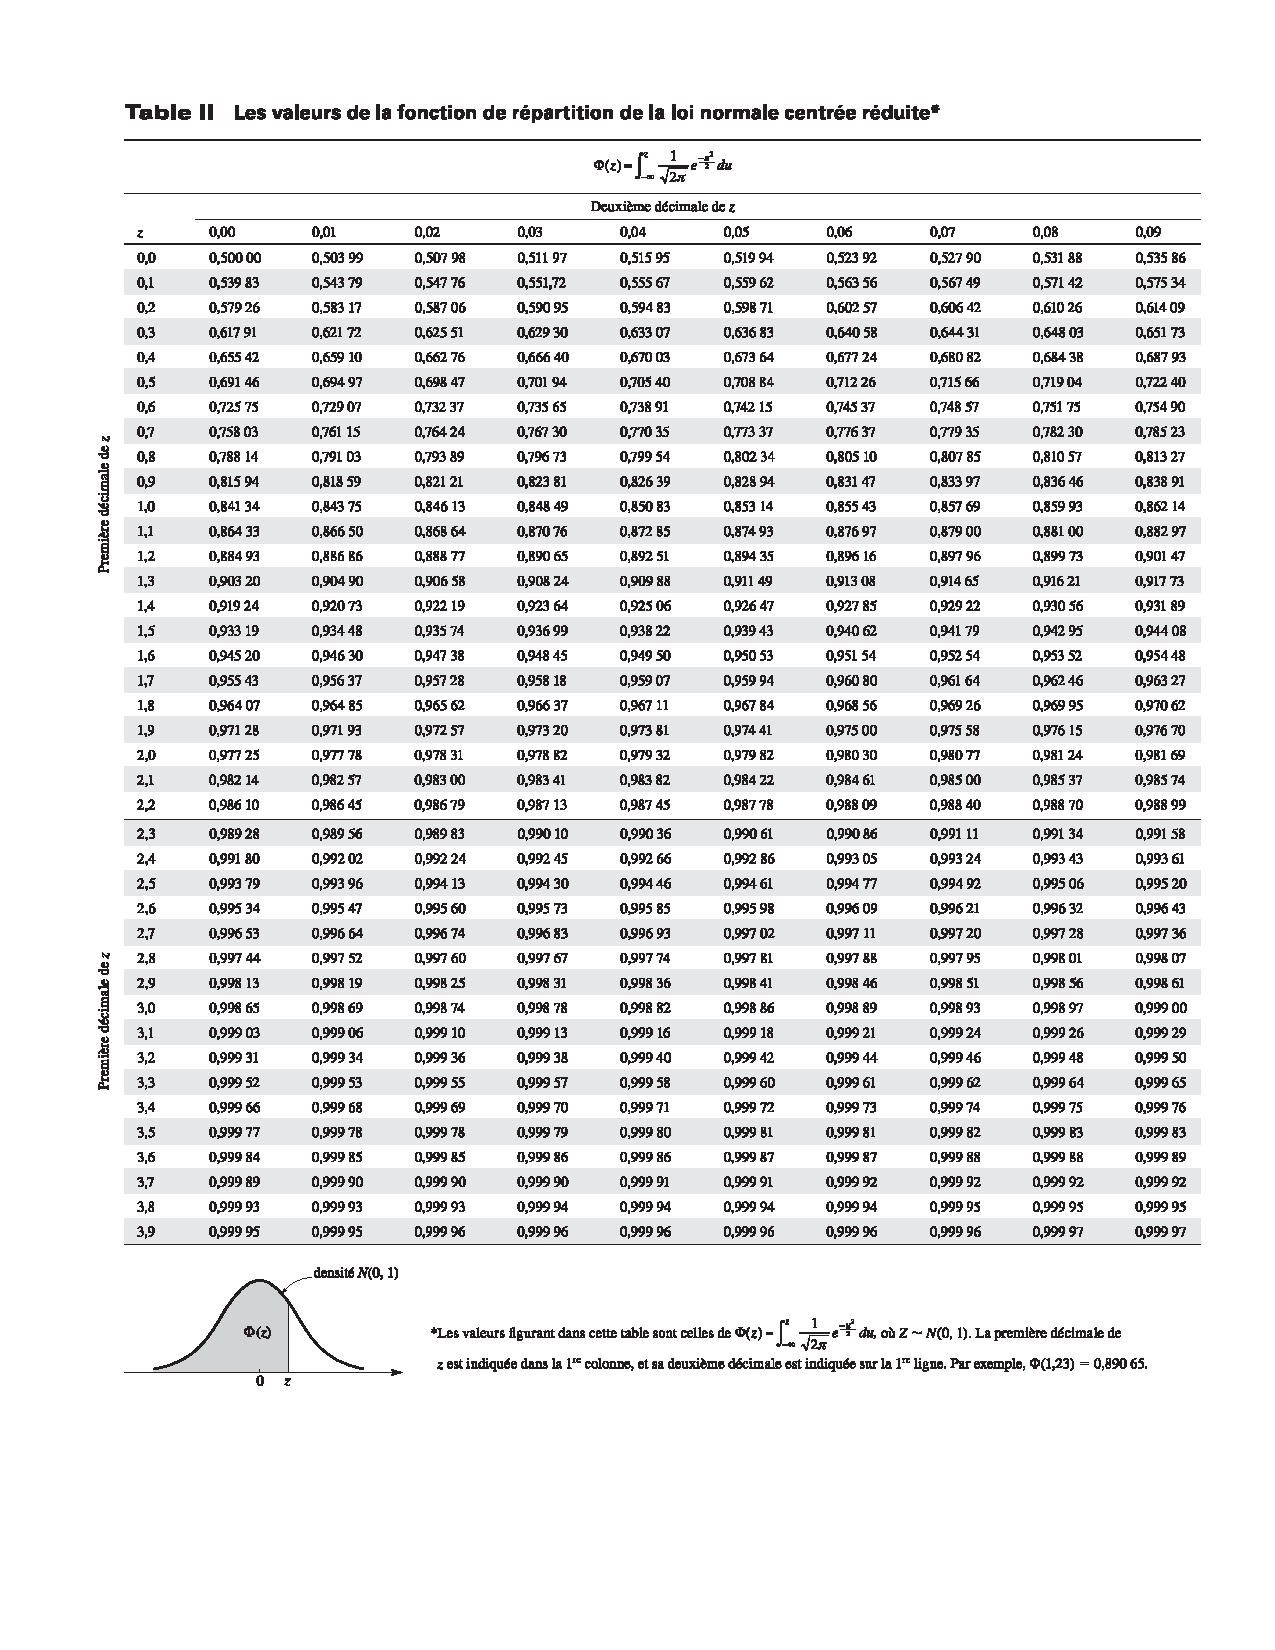
\includegraphics[trim=58 194 34 358, clip, scale=0.68]{TableNormale.pdf}
\end{center}

\end{frame}


\begin{frame}[t,label=exnorm]{Loi normale standard : utiliser la table}

On suppose que $X \sim \mathcal{N}(0,1)$.

\vspace{0.1in}
Quelle est la probabilité que $X$ soit plus petit que 1,15?

\vspace{1in}
Quelle est la probabilité que $X$ soit plus grand que 1,15?

\lienreponse{rep-ex2}
\end{frame}


\begin{frame}[t]{Loi normale standard : utiliser la table}

Quelle est la probabilité que $X$ soit entre 0,4 et 2,12?
\vspace{1in}

Quelle est la probabilité que $X$ soit plus petit que $-1{,}4$?

\lienreponse{rep-ex2}
\end{frame}


\begin{frame}[t]{Loi normale standard : utiliser la table}

Quelle est la probabilité que $X$ soit entre $-1{,}3$ et 1,98?
\vspace{1in}

Quelle est la probabilité que $|X|$ soit plus petit que 2?

\lienreponse{rep-ex2}
\end{frame}


\begin{frame}[t,label=exenvers]{Loi normale standard : lire la table à l'envers}

On peut aussi lire la table dans l'autre sens, c'est-à-dire trouver des valeurs de $x$ à partir des probabilités.
\vspace{0.1in}

Quelle est la valeur $c$ telle que $P(X < c) = 85{,}543\,\%$?
\vspace{1in}

Quelle est la valeur $c$ telle que $P(X > c) = 94{,}3\,\%$?

\lienreponse{rep-ex2}
\end{frame}


\begin{frame}{Standardisation}

Si $X \sim \mathcal{N}(\mu, \sigma^2)$ et qu'on veut calculer des probabilités pour $X$, on peut utiliser
la table de la loi normale standard grâce au processus de \alerter{standardisation} :

\begin{align*}
F_X(x)= P(X\le x)&=\int_{-\infty}^x \frac{1}{\sqrt{2\pi\sigma^2}}e^{-\frac{1}{2}(\frac{t-\mu}{\sigma})^2}dt\\[6pt]
&=\int_{-\infty}^{(x-\mu)/\sigma}\frac{1}{\sqrt{2\pi}}e^{-\frac{1}{2}z^2}\;dz\\[6pt]
&=\Phi\left(\frac{x-\mu}{\sigma}\right).
\end{align*}

\vspace{0.1in}
{\small Pour calculer la fonction de répartition d'une $\mathcal{N}(\mu, \sigma^2)$ en $x$, il suffit donc
de calculer celle de la loi normale standard en $\frac{x-\mu}{\sigma}$, par exemple à l'aide de la table.}

\end{frame}


\begin{frame}{Standardisation}

Un raisonnement semblable permet de montrer que si $$X\sim \mathcal{N}(\mu,\sigma^2),$$
alors $$Z=\frac{X-\mu}{\sigma} \sim \mathcal{N}(0,1).$$

\vspace{0.4in}
\alerter{$\Rightarrow$\ Une seule table, celle de la loi normale standard, est nécessaire!}

\end{frame}


\begin{frame}[t]{Standardisation}
Supposons que $X\sim \mathcal{N}(\mu,\sigma^2)$ et que l'on cherche
$P(a<X\le b)$.

\vspace{0.1in}
Si $Z=\frac{X-\mu}{\sigma}$, on a que $Z\sim \mathcal{N}(0,1)$. Donc
\begin{align*}
P(a<X\le b)&=P\left(\frac{a-\mu}{\sigma}<\frac{X-\mu}{\sigma}\le
\frac{b-\mu}{\sigma}\right)\\[6pt]
&=P\left(\frac{a-\mu}{\sigma}<Z\le
\frac{b-\mu}{\sigma}\right)\\[6pt]
&=\Phi\left(\frac{b-\mu}{\sigma}\right)-\Phi\left(\frac{a-\mu}{\sigma}\right).
\end{align*}
\end{frame}


\begin{frame}[t]{Standardisation}

Les problèmes de calcul de probabilités pour la loi normale se résolvent donc en deux étapes :
\begin{enumerate}
\item standardiser la v.a. d'intérêt pour obtenir des probabilités qui portent sur une $\mathcal{N}(0,1)$;
\item aller chercher les valeurs de $\Phi(\cdot)$ dans une table.
\end{enumerate}

\vspace{0.2in}
Comme la densité de la $\mathcal{N}(0,1)$ est symétrique autour de 0,
$$\Phi(-x)=1-\Phi(x) \text{ pour tout } x\in\mathbb{R}.$$
Les livres donnent donc généralement les valeurs de $\Phi(x)$ pour $x>0$ seulement.

\end{frame}


\begin{frame}[t,label=exapi]{Temps de réponse d'une API}

{\small
Le temps de réponse (en millisecondes) d'une API Web peut être vu comme une v.a.
normale de moyenne 50 et d'écart-type 10.

(i) Quelle est la probabilité qu'une requête prenne plus de 70 ms?
\vspace{1in}

(ii) Quelle proportion des requêtes prend entre 40 et 60 ms?
\vspace{1in}
}
\lienreponse{rep-ex2}
\end{frame}


\begin{frame}[t]{Temps de réponse d'une API (suite)}

{\small
(iii) Quel est le temps, disons $m_1$, tel que 97,5\,\% des requêtes ont un temps de réponse inférieur à $m_1$?
\vspace{1in}

(iv) Quel est le temps, disons $m_2$, tel que 97,5\,\% des requêtes ont un temps de réponse supérieur à $m_2$?
}
\lienreponse{rep-ex2}
\end{frame}


\begin{frame}[t]{Combinaisons linéaires de normales}

\alerter{Une combinaison linéaire de variables aléatoires normales est aussi une variable aléatoire normale},
qu'elles soient indépendantes ou non, à condition qu'elles soient \alerter{conjointement normales}
(et pas seulement normales chacune de leur côté).

\smallskip
On calcule sa moyenne et sa variance avec les formules déjà vues pour les combinaisons linéaires de
variables aléatoires.

\smallskip
Par exemple, si $X_1,X_2,\ldots,X_n$ sont des v.a. \alerter{indépendantes} et que $X_i\sim \mathcal{N}(\mu_i,\sigma^2_i)$
pour $i=1,\ldots,n$, alors
\begin{align*}
Y&=X_1+X_2+\cdots+X_n \sim \mathcal{N}\left( \sum_{i=1}^n \mu_i,\sum_{i=1}^n \sigma^2_i \right) \quad\text{et}\\[4pt]
W&=a_1X_1+\cdots+a_nX_n \sim \mathcal{N}\left( \sum_{i=1}^n a_i \mu_i,\sum_{i=1}^n a_i^2 \sigma^2_i \right).
\end{align*}

\end{frame}


\begin{frame}[t,label=exportefeuille]{Portefeuille d'actions}

{\small
Le portefeuille d'actions de votre entreprise est constitué à 20\,\% d'actions de ABC, à 30\,\%
d'actions de EFG et à 50\,\% d'actions de WXY. Les rendements des trois titres sont des v.a.
normales indépendantes de variance 0,09 et de moyenne 0,12 pour ABC, 0,15 pour EFG et 0,18 pour WXY.
Quelle est la probabilité que le rendement global de ce portefeuille dépasse 0,17?

\smallskip
(Note : le rendement global du portefeuille est la combinaison linéaire des rendements des actions
individuelles, dont les poids sont les proportions de chaque action dans le portefeuille.)
}
\lienreponse{rep-ex2}
\end{frame}


\begin{frame}[t]{Portefeuille d'actions (suite)}

\lienreponse{rep-ex2}
\end{frame}

% ----------------------------------------------------------------------------
\begin{frame}[t]{Un résultat très (très) utile}
\begin{thm}{}
Soit $X_1, X_2, \ldots, X_n$ des variables aléatoires \alerter{indépendantes} de moyenne $\mu<\infty$,
de variance $\sigma^2<\infty$ et de loi de probabilité \alerter{quelconque}.

\vspace{0.4cm}
Alors si $n$ est assez grand (généralement $n \geq 30$),

\vspace{0.4cm}
$Y\;\;=\;\;X_1+\cdots+X_n\;\;\approx\;\; \mathcal{N}(n\mu, n\sigma^2)$

\vspace{0.4cm}
$\overline X\;\;=\;\;\displaystyle\frac{X_1+\cdots+X_n}{n}\;\;\approx\;\; \mathcal{N}\left(\mu, \frac{\sigma^2}{n}\right)$
\end{thm}
Nous appelons ce théorème le \textit{théorème central limite} (TCL).

\vspace{0.1cm}
{\small Le seuil $n\ge 30$ est indicatif : une loi très asymétrique peut demander un $n$ plus grand.}
\end{frame}


\begin{frame}[t,label=quizurne]{Vrai ou faux?}

{\small
\begin{columns}[T]
\begin{column}{0.46\textwidth}
\alerter{1)} Vous tirez une boule dans une urne contenant 3 boules numérotées 1, 2 et 3.

\smallskip
\textit{La valeur de la boule tirée a la distribution de probabilité suivante :}
\end{column}
\begin{column}{0.46\textwidth}
\alerter{2)} Vous remettez la boule dans l'urne et tirez une boule à nouveau.

\smallskip
\textit{La somme des deux numéros tirés a la distribution de probabilité suivante :}
\end{column}
\end{columns}
}

\begin{columns}[T]
\begin{column}{0.46\textwidth}
\centering
\begin{tikzpicture}
\begin{axis}[loi, urne1, xlabel={Valeur de la boule}]
  \addplot[baton] coordinates {(1,0.3333) (2,0.3333) (3,0.3333)};
\end{axis}
\end{tikzpicture}
\end{column}
\begin{column}{0.46\textwidth}
\centering
\begin{tikzpicture}
\begin{axis}[loi, urne2, xlabel={Somme des deux numéros}]
  \addplot[baton] coordinates {(2,0.2) (3,0.2) (4,0.2) (5,0.2) (6,0.2)};
\end{axis}
\end{tikzpicture}
\end{column}
\end{columns}

\lienreponse{rep-ex3}
\end{frame}


\begin{frame}[t,label=excentre]{Consommation d'un centre de données}

{\small
Supposons que les consommations quotidiennes d'électricité des 100 serveurs d'un centre de données
peuvent être vues comme des v.a. indépendantes de moyenne 10 kWh et d'écart-type 5 kWh.

Quelle est la probabilité approximative que la consommation quotidienne totale de ces 100 serveurs
dépasse la capacité de 1100 kWh de l'alimentation électrique du centre?}

\vspace{3.2cm}

\lienreponse{rep-ex3}
\end{frame}


\begin{frame}[t]{Consommation d'un centre de données (solution)}

\lienreponse{rep-ex3}
\end{frame}

% ============================================================================
\section{Application : approximation de la loi binomiale par la loi normale}

\begin{frame}[t]{Idée générale}

Une v.a. binomiale peut s'écrire comme une somme de v.a. indépendantes :
\vspace{1in}

On peut donc approximer sa distribution par une loi normale, pourvu que $n$
soit assez grand (par exemple, $np\ge 5$ et $n(1-p)\ge 5$) :

\end{frame}


\begin{frame}[t,label=exclassif]{Erreurs d'un classificateur}

Un modèle de classification d'images se trompe sur 10\,\% des images, indépendamment d'une
image à l'autre. On lui soumet un lot de 100 images. Quelle est la probabilité qu'il fasse plus
de 5 erreurs?

\lienreponse{rep-ex3}
\end{frame}


\begin{frame}[t]{Erreurs d'un classificateur (suite)}

Quelle est la probabilité que le modèle fasse exactement 5 erreurs?

\lienreponse{rep-ex3}
\end{frame}


\begin{frame}[t]{Correction pour la continuité}

La loi binomiale est discrète, mais la loi normale est continue : on doit donc faire une
\alerter{correction pour la continuité}.

\vspace{0.2in}
Pour calculer $P(X=a)$, on calcule $P(a-0{,}5 \leq X \leq a+0{,}5)$.

\vspace{0.2in}
De même pour les autres probabilités :

\vspace{0.05in}
\begin{center}
\begin{tabular}{l}
$P(X \leq a) \approx$ \\[14pt]
$P(X < a) \approx$ \\[14pt]
$P(X \geq a) \approx$ \\[14pt]
$P(X > a) \approx$
\end{tabular}
\end{center}

\end{frame}


\begin{frame}[t]{Erreurs d'un classificateur (suite), avec correction}

Un modèle de classification d'images se trompe sur 10\,\% des images, indépendamment d'une
image à l'autre. On lui soumet un lot de 100 images. Quelle est la probabilité qu'il fasse plus
de 5 erreurs?

\lienreponse{rep-ex3}
\end{frame}

% ============================================================================
\section{Compléments : loi de Weibull}

\begin{frame}[t]{Loi de Weibull}

La loi de Weibull permet de modéliser une situation où la probabilité qu'un événement survienne
n'est pas constante dans le temps, contrairement à la loi exponentielle. Par exemple, la
probabilité qu'un appareil tombe en panne dans un instant donné ne reste souvent pas constante :
elle augmente avec l'âge de l'appareil.

\vspace{0.2in}
Le rythme de cette augmentation est contrôlé par un des paramètres de la loi (le paramètre de forme).

\end{frame}


\begin{frame}{Loi de Weibull}

Si $X$ suit une loi de Weibull$(\delta,\beta,\gamma)$, alors
$$f(x)=\left\{\begin{array}{ll}
\frac{\beta}{\delta}\left(\frac{x-\gamma}{\delta}\right)^{\beta-1}
\exp\left\{-\left(\frac{x-\gamma}{\delta}\right)^\beta\right\}, & x>\gamma\\
0, & \text{sinon}.\end{array}\right.$$

\vspace{0.2in}
On appelle $\beta$ le « paramètre de forme » et $\delta$ le « paramètre d'échelle ».

\vspace{0.4in}
Si $\gamma=0$ et $\beta=1$, on retrouve la loi exponentielle de moyenne $\delta$!

\end{frame}


\begin{frame}{Loi de Weibull : fonction de répartition}

En posant $u=\{(s-\gamma)/\delta\}^\beta$ dans $\int_{-\infty}^xf(s)\;ds$, on trouve
$$F(x)=\left\{\begin{array}{ll}
0, & x<\gamma\\
1-\exp\left\{-\left(\frac{x-\gamma}{\delta}\right)^\beta\right\}, & x\ge\gamma.
\end{array}\right.$$

\vspace{0.4in}
L'espérance et la variance de la loi de Weibull ont des formes un peu compliquées et ne sont pas à l'étude.

\end{frame}


\begin{frame}[t,label=exsolaire]{Panneaux solaires}

{\small
Les panneaux solaires qui alimentent un centre de données ont des durées de vie (en années)
indépendantes, toutes de loi de Weibull$(20,2,0)$. Ces panneaux sont vendus avec une garantie
de 5 ans. Quelle est la probabilité qu'un panneau ne dure pas jusqu'à la fin de sa garantie?}
\lienreponse{rep-ex4}
\end{frame}


\begin{frame}[t]{Panneaux solaires (suite)}

{\small
S'il en coûte 1000\,\$ pour remplacer un panneau qui ne survit pas jusqu'à la fin de la garantie
et que l'on vend 500 de ces panneaux, quel est le coût total espéré de la garantie?}
\lienreponse{rep-ex4}
\end{frame}


\begin{frame}[t,label=exportable]{Durée de vie d'un ordinateur portable}

{\small
La durée de vie de votre ordinateur portable (en années) suit une loi de Weibull avec $\beta=3$,
$\delta=4$ et $\gamma=0$.

Quelle est la probabilité que votre portable fonctionne encore au moins 3 années de plus
(i) s'il est neuf? (ii) s'il a 2 ans?
}
\lienreponse{rep-ex4}
\end{frame}


\begin{frame}[t]{Durée de vie d'un ordinateur portable (suite)}

{\small
Quelle est la durée de vie médiane de ces portables, c'est-à-dire le 50\textsuperscript{e} centile
de la distribution (la durée telle que 50\,\% des portables durent moins longtemps et 50\,\% durent
plus longtemps)?}
\lienreponse{rep-ex4}
\end{frame}

% ============================================================================
\section{Réponses des exemples}

\begin{frame}[t,label=rep-ex1]{Réponses des exemples (1/4)}
\footnotesize
\begin{itemize}\itemsep4pt
\item \retour{exfreq}{Fréquence d'un processeur} : $X\sim\mathcal{U}(1{,}5\,;2)$~;
$P(X>1{,}8)=\frac{2-1{,}8}{2-1{,}5}=0{,}4$~; $E(X)=1{,}75$ GHz.
\item \retour{excommits}{Commits sur un dépôt} : $X\sim\text{Exp}(1/3)$~; $P(X>6)=e^{-2}\approx0{,}1353$~;
nombre de commits en 15 h $\sim\text{Poisson}(5)$, d'où $P(4\text{ commits})=e^{-5}5^4/4!\approx0{,}1755$.
\item \retour{exserveur}{Serveur sans plantage} : par l'absence de mémoire,
$P(X>1500\,|\,X>500)=P(X>1000)=e^{-1}\approx0{,}3679$.
\item \retour{expirate}{Pirate informatique} : $X\sim\text{Gamma}(3,1/15)$~; $E(X)=45$ minutes~;
$V(X)=675$ minutes$^2$.
\item \textbf{Pirate informatique (suite)} : nombre de mots de passe craqués en 20 minutes
$\sim\text{Poisson}(4/3)$~; $P(W=2)=e^{-4/3}(4/3)^2/2!\approx0{,}2343$.
\end{itemize}
\end{frame}


\begin{frame}[t,label=rep-ex2]{Réponses des exemples (2/4)}
\footnotesize
\begin{itemize}\itemsep4pt
\item \retour{exnorm}{Loi normale standard : utiliser la table} : $P(X<1{,}15)=\Phi(1{,}15)=0{,}8749$~;
$P(X>1{,}15)=0{,}1251$~; $P(0{,}4<X<2{,}12)=0{,}3276$~; $P(X<-1{,}4)=1-\Phi(1{,}4)=0{,}0808$~;
$P(-1{,}3<X<1{,}98)=0{,}8794$~; $P(|X|<2)=2\Phi(2)-1=0{,}9545$.
\item \retour{exenvers}{Lire la table à l'envers} : $c=1{,}06$~; $c=-1{,}58$.
\item \retour{exapi}{Temps de réponse d'une API} : (i) $P(X>70)=1-\Phi(2)=0{,}0228$~;
(ii) $P(40<X<60)=\Phi(1)-\Phi(-1)=0{,}6827$~;
(iii) $m_1=50+1{,}96\times10=69{,}6$ ms~; (iv) $m_2=50-1{,}96\times10=30{,}4$ ms.
\item \retour{exportefeuille}{Portefeuille d'actions} : $R=0{,}2A+0{,}3E+0{,}5W\sim\mathcal{N}(0{,}159\,;0{,}0342)$~;
$P(R>0{,}17)=P(Z>0{,}0595)\approx0{,}476$.
\end{itemize}
\end{frame}


\begin{frame}[t,label=rep-ex3]{Réponses des exemples (3/4)}
\footnotesize
\begin{itemize}\itemsep4pt
\item \retour{quizurne}{Vrai ou faux?} : 1) vrai, chaque valeur a probabilité $1/3$~;
2) faux : les sommes $2,3,4,5,6$ ont probabilités $1/9$, $2/9$, $3/9$, $2/9$, $1/9$.
\item \retour{excentre}{Consommation d'un centre de données} : par le TCL, $Y\approx\mathcal{N}(1000,2500)$~;
$P(Y>1100)\approx P(Z>2)=0{,}0228$.
\item \retour{exclassif}{Erreurs d'un classificateur} : $X\sim\text{Bin}(100\,;0{,}1)$, $E(X)=10$, $V(X)=9$~;
valeur exacte $P(X>5)\approx0{,}9424$~; sans correction, $P(X>5)\approx P(Z>-1{,}667)=\Phi(1{,}667)\approx0{,}9522$.
\item \textbf{Erreurs d'un classificateur (suite)} : sans correction, $P(X=5)\approx0$ (d'où le besoin
d'une correction pour la continuité)~; avec correction, $P(4{,}5\le X\le5{,}5)\approx0{,}033$
(valeur exacte $0{,}0339$).
\item \textbf{Avec correction} : $P(X>5)=P(X\ge6)\approx P(X\ge5{,}5)=P(Z\ge-1{,}5)=\Phi(1{,}5)\approx0{,}9332$.
\end{itemize}
\end{frame}


\begin{frame}[t,label=rep-ex4]{Réponses des exemples (4/4) : loi de Weibull}
\footnotesize
\begin{itemize}\itemsep4pt
\item \retour{exsolaire}{Panneaux solaires} : $P(X<5)=F(5)=1-e^{-(5/20)^2}=1-e^{-0{,}0625}\approx0{,}0606$.
\item \textbf{Panneaux solaires (suite)} : coût total espéré
$=500\times1000\,\$\times0{,}0606\approx30\,294\,\$$.
\item \retour{exportable}{Durée de vie d'un ordinateur portable} : (i) $P(X\ge3)=e^{-(3/4)^3}\approx0{,}6558$~;
(ii) $P(X\ge5\,|\,X\ge2)=e^{-(5/4)^3}/e^{-(2/4)^3}=e^{-1{,}828125}\approx0{,}1607$.
\item \textbf{Durée de vie d'un ordinateur portable (suite)} : $m$ tel que $(m/4)^3=\ln2$,
d'où $m\approx3{,}54$ ans.
\end{itemize}
\end{frame}


\begin{frame}{Bibliographie}
 	Ce document est rédigé avec Beamer ainsi qu'une classe .cls fournie par Jérôme Soucy. Les diapositives sont adaptées des diapositives créées par Anne-Sophie Charest
 pour le cours STT-1000 ainsi que celles créées par Thierry Duchesne et Emmanuelle Reny-Nolin pour le cours STT-1900. La table de la loi normale provient de ces mêmes diapositives.
 	\printbibliography
 	\vfill
 	\footnotesize Pour signaler une erreur dans ce document, veuillez écrire à l'adresse :~\href{mailto:julien.miron@mat.ulaval.ca}{julien.miron@mat.ulaval.ca}.
 \end{frame}

\end{document}
